

\chapter{编队网络模型和拓扑分析}
\label{chap:2}

\section{机器人编队网络模型}
在多机器人编队控制过程中,每个机器人个体都具有自主行动能力。尤其在实现分布式控制算法时,每个个体机器人需要具有独立的决策与执行能力。因此,机器人个体运动模型对编队的控制至关重要。另外在应用编队控制算法对整个编队系统进行控制从而实现特定任务时,对整体编队网络拓扑模型的掌握也是必不可少。编队网络拓扑模型是对整体编队网络拓扑分析与拓扑控制的基础\supercite{张飞2010}。

\subsection{机器人个体运动模型}
假设在$N$维空间内,机器人$i$的位置和速度分别表示为$p_i \in R^N$和$v_i \in R^N$。则机器人个体运动模型可以表示如下:\\
\begin{equation}
	\left\{
	\begin{aligned}
		\dot{p_i} & = v_i \\
		\dot{v_i} & = u_i^e + u_i^o
	\end{aligned}
	, i=1,2,\dots,n,
	\right.
\end{equation}
其中$u_i^e$表示外部对机器人的控制输入,$u_i^o$表示其他机器人对机器人$i$的影响。$u_i^e$可简单表示为:\\
\begin{equation}
	u_i^e = f(p_i,v_i), i=1,2,\dots,n
\end{equation}
若考虑障碍环境中,则$u_i^e$可表示为:\\
\begin{equation}
	u_i^e = f_a(p_i,v_i) + f_r(p_i,v_i), i=1,2,\dots,n
\end{equation}
其中,$f_a(p_i,v_i)$为目标对机器人的吸引力,$f_r(p_i,v_i)$为障碍物对机器人的排斥力。如果已知目标点的位置$T$和机器人当前位置的期望速度$v(t)$,则$f_a(p_i,v_i)$可以表示为:\\
\begin{equation}
	f_a(p_i,v_i) = a_a(T-p_i) + a_m(v(t)-v_i), i=1,2,\dots,n
\end{equation}
$a_a,a_m$分别为位置和速度的增益系数,且满足$a_a,a_m > 0$。

假设环境中存在一球形障碍物,其中心点位于$O$,半径为$r_0$,则排斥力$f_r(p_i,v_i)$可表示为:\\
\begin{equation}
	f_r(p_i,v_i) = \begin{cases}
		\frac{a_0}{{(\lvert\lvert p_i-O \rvert\rvert -r_0)}^2} \cdot \vec{r}_t, & \lvert\lvert O-p_i \rvert\rvert \leq r_0 + R_s \\
		0, &  \lvert\lvert O-p_i \rvert\rvert > r_0 + R_s
	\end{cases}
\end{equation}
其中$a_0$为排斥系数,$R_s$为人为设置的障碍物有效作用半径。$\vec{r}_t$为排斥力的方向,即$\vec{r}_t = \vec{Op_i}/\lvert\lvert\vec{Op_i}\rvert\rvert$。

\subsection{多机器人编队网络拓扑模型}
本文的拓扑结构采用基于图论的网络拓扑。假设机器人编队中有$n$个机器人,$n$个机器人组成的编队网络用$G=(V,E)$表示,其中$V$表示图中节点的集合,$E$表示节点间边的集合。每个节点$v_i\in V, i=1,2,\dots,n$表示机器人$i$, $(v_i,v_j)\in E, i,j=1,2,\dots,n$表示机器人$i,j$之间的链接。利用矩阵$A=(a_{ij}),a_{ij} \in R^{n \times n}$表示网络拓扑的耦合关系,其中\\
\begin{equation}
	a_{ij}=a_{ji} =
	\begin{cases}
		1, & (v_i,v_j) \in E \\
		0, & (v_i,v_j) \notin E
	\end{cases}
	, i,j = 1,2,\dots\dots,n, i \neq j
\end{equation}
$a_{ij} = a){ji} = 1$ 表示机器人$i,j$之间存在有效链接,否则不存在链接。耦合矩阵对角线上的元素$a_{ij} = -\sum_{i=1,i \neq j}^n a_{ij}$。规定与机器人$i$存在有效连接的机器人属于机器人$i$的邻居。则定义机器人$i$的邻居集合$N_e(i)$为:\\
\begin{equation}
	N_e(i) = \left\{ \forall j, j \neq i \wedge a_{ij}=1 \right\}
\end{equation}
机器人$i$的度为:\\
\begin{equation}
	d_i = \sum_{j \in N_e(i)} a_{ij}
\end{equation}
由此可知,耦合矩阵对角线上的元素$a_{ii} = -d_i$。

多机器人编队网络拓扑多采用$K$邻居模型\supercite{xue2004number}描述。在K邻居模型中,每个机器人的度$d_i \leq K, i=1,2, \dots ,n$。图2-1展示了几种常见的$K$邻居网络拓扑模型。

\begin{figure*}[!htbp]
	\centering
	\begin{tabular}{lr}
		\subfigure[K=3]{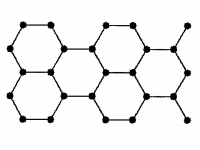
\includegraphics[width=5cm,height=4cm]{chapter2/figure2-1a.png}} &
		\subfigure[K=4]{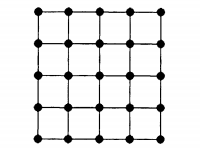
\includegraphics[width=5cm,height=4cm]{chapter2/figure2-1b.png}} \\
		\subfigure[K=6]{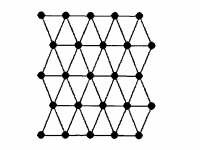
\includegraphics[width=5cm,height=4cm]{chapter2/figure2-1c.png}} &
		\subfigure[K=8]{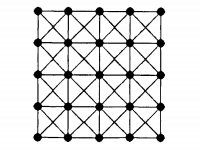
\includegraphics[width=5cm,height=4cm]{chapter2/figure2-1d.png}} \\
	\end{tabular}
\end{figure*}
